% !Tex Program = xelatex
% -*-coding: utf-8 -*-
\documentclass[12pt,onecolumn]{article}

% 中文
\usepackage[BoldFont,SlantFont]{xeCJK}
\xeCJKsetemboldenfactor{1}%只对随后定义的CJK字体有效
\setCJKfamilyfont{hei}{SimHei}
\xeCJKsetemboldenfactor{4}
\setCJKfamilyfont{song}{SimSun}
\xeCJKsetemboldenfactor{4}
\setCJKfamilyfont{fs}{FangSong}
\setCJKfamilyfont{kai}{KaiTi}
\setCJKfamilyfont{li}{LiSu}
\setCJKfamilyfont{xw}{STXinwei}
\setCJKmainfont{SimSun}

\newcommand{\hei}{\CJKfamily{hei}}      % 黑体
\newcommand{\song}{\CJKfamily{song}}    % 宋体   (Windows 自带simsun.ttf)
\newcommand{\fs}{\CJKfamily{fs}}        % 仿宋体 (Windows 自带simfs.ttf)
\newcommand{\kai}{\CJKfamily{kai}}      % 楷体   (Windows 自带simkai.ttf)
\newcommand{\li}{\CJKfamily{li}}        % 隶书   (Windows自带simli.ttf)
\newcommand{\xw}{\CJKfamily{xw}}        % 隶书   (Windows自带simli.ttf)

% \AmSTeX\ 宏包,用来排出更加漂亮的公式。
\usepackage{amsmath}
% 定理类环境宏包,其中 \pkg{amsmath} 选项用来兼容 \AmSTeX\ 的宏包
\usepackage[amsmath,thmmarks,hyperref]{ntheorem}
\usepackage{amssymb}
% 添加字体
\usepackage[defaultsups]{newtxtext}
\usepackage{newtxmath}
\usepackage{courier}
% 图形支持宏包
\usepackage{graphicx}
% 插入pdf
\usepackage{pdfpages}
\includepdfset{fitpaper=true}
% 更好的列表环境。
\usepackage{enumitem}       %使用enumitem宏包,改变列表项的格式
\usepackage{environ}
% 禁止 \LaTeX 自动调整多余的页面底部空白,并保持脚注仍然在底部。
% 脚注按页编号。
\usepackage[bottom,perpage,hang]{footmisc}
\raggedbottom
% 脚注格式。
\usepackage{pifont}
% 表格控制
\usepackage{longtable}
\usepackage{booktabs}
% 参考文献引用宏包
\usepackage[sort&compress]{natbib}
% 生成有书签的 pdf 及其开关,请结合 gbk2uni 避免书签乱码。
\usepackage{hyperref}
\hypersetup{
	CJKbookmarks=true,
	linktoc=all,
	bookmarksnumbered=true,
	bookmarksopen=true,
	bookmarksopenlevel=1,
	breaklinks=true,
	colorlinks=false,
	plainpages=false,
	pdfborder=0 0 0}
% 设置 url 样式,与上下文一致
\urlstyle{same}
% 版芯设置
\usepackage{geometry}
\geometry{
	centering,
	text={150true mm,236true mm},
	left=30true mm,
	head=5true mm,
	headsep=2true mm,
	footskip=0true mm,
	foot=5.2true mm
}
% 利用 \pkg{fancyhdr} 设置页眉页脚。
\usepackage{fancyhdr}
% 其他包,表格、数学符号包
\usepackage{tabularx}
\usepackage{varwidth}
% 此处changepage环境用来控制索引页面的左右边距,规范中给出的示例的边距要大于正文。
\usepackage{changepage}
% 多栏结构在文中用begin{multicols}{2}end{multicols}
\usepackage{multicol,multienum}
% 允许上一个section的浮动图形出现在下一个section的开始部分,还提供\FloatBarrier命
% 令,使所有未处理的浮动图形立即被处理
\usepackage[below]{placeins}
% 支持子图 %centerlast 设置最后一行是否居中
\usepackage{subfigure}
% 支持双语标题
\usepackage[subfigure]{ccaption}
% 根据我工规定,正文小四号 (12bp) 字,行距为固定值3--4mm。
\renewcommand\normalsize{%
	% \@setfontsize\normalsize{12bp}{\ifhit@glue 20.50398bp \@plus 2.83465bp \@minus 0bp\else 20.50398bp\fi}%
	\abovedisplayskip=8pt
	\abovedisplayshortskip=8pt
	\belowdisplayskip=\abovedisplayskip
	\belowdisplayshortskip=\abovedisplayshortskip}
% 根据习惯定义字号。用法:\cs{hit@def@fontsize}\marg{字号名称}\marg{磅数}避免了
% 字号选择和行距的紧耦合。所有字号定义时为单倍行距,并提供选项指定行距倍数。
\def\hit@def@fontsize#1#2{%
	\expandafter\newcommand\csname #1\endcsname[1][1.3]{%
		\fontsize{#2}{##1\dimexpr #2}\selectfont}}
\hit@def@fontsize{dachu}{58bp}
\hit@def@fontsize{chuhao}{42bp}
\hit@def@fontsize{xiaochu}{36bp}
\hit@def@fontsize{yihao}{26bp}
\hit@def@fontsize{xiaoyi}{24bp}
\hit@def@fontsize{erhao}{22bp}
\hit@def@fontsize{xiaoer}{18bp}
\hit@def@fontsize{sanhao}{16bp}
\hit@def@fontsize{xiaosan}{15bp}
\hit@def@fontsize{sihao}{14bp}
\hit@def@fontsize{banxiaosi}{13bp}
\hit@def@fontsize{xiaosi}{12bp}
\hit@def@fontsize{dawu}{11bp}
\hit@def@fontsize{wuhao}{10.5bp}
\hit@def@fontsize{xiaowu}{9bp}
\hit@def@fontsize{liuhao}{7.5bp}
\hit@def@fontsize{xiaoliu}{6.5bp}
\hit@def@fontsize{qihao}{5.5bp}
\hit@def@fontsize{bahao}{5bp}
% 利用 \pkg{enumitem} 命令调整默认列表环境间的距离,以符合中文习惯。
\setlist{nosep}
% 允许太长的公式断行、分页等。
\allowdisplaybreaks[4]
\predisplaypenalty=0  %公式之前可以换页,公式出现在页面顶部
\postdisplaypenalty=0
% 公式编号设置
\renewcommand{\theequation}{\arabic{section}.\arabic{equation}}
% 定理标题使用黑体,正文使用宋体,冒号隔开。
\theorembodyfont{\normalfont}
\theoremheaderfont{\normalfont\hei}
\theoremsymbol{\ensuremath{\square}}
\newtheorem*{proof}{证明}
\theoremstyle{plain}
\theoremsymbol{}
\theoremseparator{}
\newtheorem{assumption}{假设}[section]
\newtheorem{definition}{定义}[section]
\newtheorem{proposition}{命题}[section]
\newtheorem{lemma}{引理}[section]
\newtheorem{theorem}{定理}[section]
\newtheorem{axiom}{公理}[section]
\newtheorem{corollary}{推论}[section]
\newtheorem{exercise}{练习}[section]
\newtheorem{example}{例}[section]
\newtheorem{remark}{注释}[section]
\newtheorem{problem}{问题}[section]
\newtheorem{conjecture}{猜想}[section]
\newtheorem{solution}{解}[section]
% 各种单位
\usepackage{siunitx}
\sisetup{group-minimum-digits=4, group-separator= \hspace{0.25em}}
\sisetup{detect-weight,detect-mode,detect-family}
% 处理数学公式中的黑斜体的宏包
\usepackage{bm}
% 不同于 \mathcal \mathfrak 之类的英文花体字体
\usepackage{mathrsfs}
% 支持彩色
\usepackage{xcolor}
\definecolor{colorzero}{rgb}{0, 0, 0}
\definecolor{colorone}{rgb}{1, 0, 0}
\definecolor{colortwo}{rgb}{0, 0, 1}
\definecolor{colorthree}{rgb}{0, 1, 0}
% 图形和表格的控制旋转
\usepackage{rotating}
% 算法的宏包,注意宏包兼容性,先后顺序为float、hyperref、algorithm(2e),否则无法
% 生成算法列表。
\usepackage[algoruled,linesnumbered]{algorithm2e}
% 排版源码所使用的环境。
\usepackage{listings}
\lstset{
	breaklines  = true,
	captionpos  = b,
	tabsize     = 2,
	numbers     = left,
	columns     = flexible,
	keepspaces  = true,
	% commentstyle = \color[RGB]{0,128,0},
	% keywordstyle = \color[RGB]{0,0,255},
	basicstyle   = \small\ttfamily,
	rulesepcolor = \color{red!20!green!20!blue!20},
	showstringspaces = false,
}

% 作图
\usepackage{tikz}
\usetikzlibrary{arrows,automata}

% 首行缩进
\usepackage{indentfirst}
\setlength{\parindent}{2em}

\usepackage{float}
\usepackage{diagbox}

% 最后定义一些常见的数学公式样式。
\newcommand{\theVector}[1]{\bm{#1}}
\newcommand{\theMatrix}[1]{\mathbb{#1}}
\newcommand{\theSet}[1]{\mathcal{#1}}
\newcommand{\theDirected}[1]{{\overrightarrow{#1}}}
\newcommand{\theUndirected}[1]{{\overline{#1}}}
\newcommand{\theNetwork}[1]{\mathscr{#1}}
\newcommand{\theNode}[1]{{\text{#1}}}
\newcommand{\theDirectedEdge}[2]{{\overrightarrow{{#1}{#2}}}}
\newcommand{\theUndirectedEdge}[2]{{\overline{{#1}{#2}}}}

\graphicspath{{figures/}}

\pagestyle{fancy}
\fancyhead[L]{\song\xiaowu[0]{哈尔滨工业大学}}
\fancyhead[R]{\song\xiaowu[0]{形式语言与自动机}}
\fancyfoot[C]{\xiaowu-~\thepage~-}

% \renewcommand{\thesection}{}
% \renewcommand{\thesubsection}{}
\renewcommand{\today}{\number\year{年}\number\month{月}\number\day{日}}
\renewcommand{\figurename}{图}
\renewcommand{\tablename}{表}

\title{形式语言与自动机~作业四}
\author{cycleke}
\date{}

\begin{document}
\maketitle
\thispagestyle{fancy}

\section{第一题}
Design a PDA (Diagram) to accept each of the following languages.
You may accept either by final state or by empty stack,
whichever is more convenient.
\subsection{(a)}
The set of all strings of 0's and 1's such that
no prefix has more 1’s than 0's.

\begin{solution}
 此 PDA 使用终结状态方式。
 \begin{figure}[H]
 \centering
 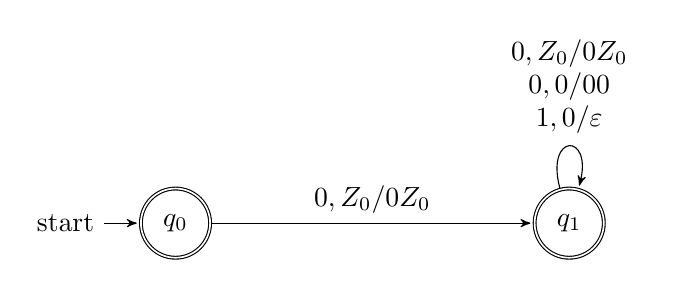
\begin{tikzpicture}[>=stealth',shorten >=1pt,auto,node distance=5cm]
 \node[state,initial,accepting] (q0) {$q_0$};
 \node[state,accepting,right of=q0] (q1) {$q_1$};

 \path[->] (q0)
 edge node {$0, Z_0 / 0Z_0$} (q1)
 (q1)
 [loop above] edge node {$
 \begin{array}{c}
 0, Z_0 / 0Z_0 \\
 0, 0 / 00     \\
 1, 0 / \varepsilon
 \end{array}
 $} (q1);
 \end{tikzpicture}
 \caption{第一题 (a)}
 \end{figure}
\end{solution}

\subsection{(b)}
The set of all strings of 0's and 1's with twice as many 0's as 1's.

\begin{solution}
 此 PDA 使用空栈方式。
 \begin{figure}[H]
 \centering
 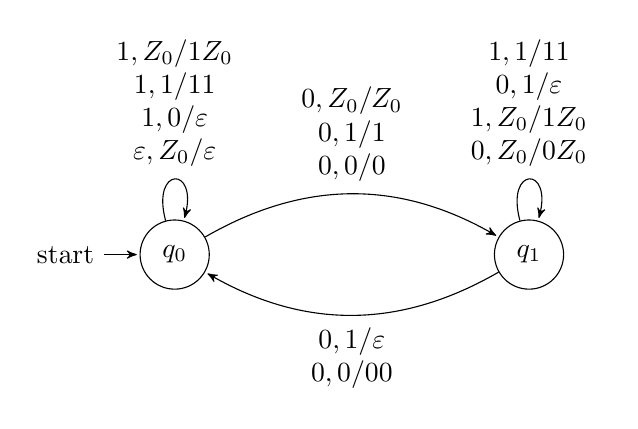
\begin{tikzpicture}[>=stealth',shorten >=1pt,auto,node distance=4.5cm]
 \node[state,initial] (q0) {$q_0$};
 \node[state,right of=q0] (q1) {$q_1$};

 \draw[->] (q0) edge [bend left] node {$
 \begin{array}{c}
 0, Z_0 / Z_0 \\
 0, 1 / 1     \\
 0, 0 / 0
 \end{array}
 $} (q1)

 (q1) edge [bend left] node {$
 \begin{array}{c}
 0, 1 / \varepsilon \\
 0, 0 / 00
 \end{array}
 $} (q0)

 (q0) [loop above] edge node {$
 \begin{array}{c}
 1, Z_0 / 1Z_0      \\
 1, 1 / 11          \\
 1, 0 / \varepsilon \\
 \varepsilon, Z_0 / \varepsilon
 \end{array}$} (q0)

 (q1) edge node {$
 \begin{array}{c}
 1, 1 / 11          \\
 0, 1 / \varepsilon \\
 1, Z_0 / 1Z_0      \\
 0, Z_0 / 0Z_0
 \end{array}$} (q1);
 \end{tikzpicture}
 \caption{第一题 (b)}
 \end{figure}

 其中$q_0$表示没有 0 与栈最上方的 1 匹配,
 而$q_1$表示有一个 0 与栈最上方的 1 匹配。
\end{solution}

\subsection{(c)}
$\{a^i b^j c^k | i \neq j~or~j \neq k\}$.

\begin{solution}
 此 PDA 使用终结状态方式。
 \begin{figure}[H]
 \centering
 \begin{tikzpicture}[>=stealth',shorten >=1pt,auto,node distance=2.8cm]
 \node[initial,state] (q0) {$q_0$};
 \node[state,above right of=q0] (q1) {$q_1$};
 \node[state,right of=q1] (q2) {$q_2$};
 \node[state,accepting,right of=q2] (q3) {$q_3$};
 \node[state,below right of=q0] (q4) {$q_4$};
 \node[state,right of=q4] (q5) {$q_5$};
 \node[state,right of=q5] (q6) {$q_6$};
 \node[state,accepting,right of=q6] (q7) {$q_7$};

 \path[->] (q0)
 edge node {$\varepsilon, Z_0 / Z_0$} (q1)
 edge node [below left] {$\varepsilon, Z_0 / Z_0$} (q4)
 (q1) edge node {$
 \begin{array}{c}
 \varepsilon, Z_0 / Z_0 \\
 \varepsilon, a / a
 \end{array}$} (q2)
 (q2) edge node {$
 \begin{array}{c}
 \varepsilon, a / a \\
 \varepsilon, b / b
 \end{array}$} (q3)
 (q4) edge node {$
 \begin{array}{c}
 \varepsilon, Z_0 / Z_0 \\
 \end{array}$} (q5)
 (q5) edge node {$
 \begin{array}{c}
 \varepsilon, Z_0 / Z_0 \\
 \varepsilon, b / b
 \end{array}$} (q6)
 (q6) edge node {$
 \begin{array}{c}
 \varepsilon, b / b \\
 \varepsilon, c / c
 \end{array}$} (q7)

 (q1) edge [loop above] node {$
 \begin{array}{c}
 a, Z_0 / aZ_0 \\
 a, a / aa
 \end{array}$} (q1)
 (q2) edge [loop above] node {$
 \begin{array}{c}
 b, Z_0 / bZ_0 \\
 b, b / bb     \\
 b, a / \varepsilon
 \end{array}$} (q2)
 (q3) edge [loop above] node {$
 \begin{array}{c}
 c, b / b \\
 c, a / a
 \end{array}$} (q3)
 (q4) edge [loop below] node {$
 \begin{array}{c}
 a, Z_0 / Z_0
 \end{array}$} (q4)
 (q5) edge [loop below] node {$
 \begin{array}{c}
 b, Z_0 / bZ_0 \\
 b, b / bb
 \end{array}$} (q5)
 (q6) edge [loop below] node {$
 \begin{array}{c}
 c, Z_0 / cZ_0 \\
 c, c / cc     \\
 c, b / \varepsilon
 \end{array}$} (q6)
 \end{tikzpicture}
 \caption{第一题 (c)}
 \end{figure}
\end{solution}

\section{第二题}
Let $\Sigma = \{0, 1\}$.
Suppose $w$ is a non-null string of even length so that
$w$ can be written as $uxyv$ with $x, y$ in $\Sigma$ and $|u| = |v|$.
Then we will say that $xy$ is the middle of $w$.
For example, in the string $00110011$ we have $10$ as its middle.
Let $L \subseteq \Sigma^*$ be given by:
$w$ is in $L$ if and only if
it is of non-null string of even length and its middle is $00$ or $11$.

Show that $L$ is a context free language by
constructing a (non-deterministic) push-down automaton that accepts $L$.

\begin{solution}
 此 PDA 使用空栈方式。
 \begin{figure}[H]
 \centering
 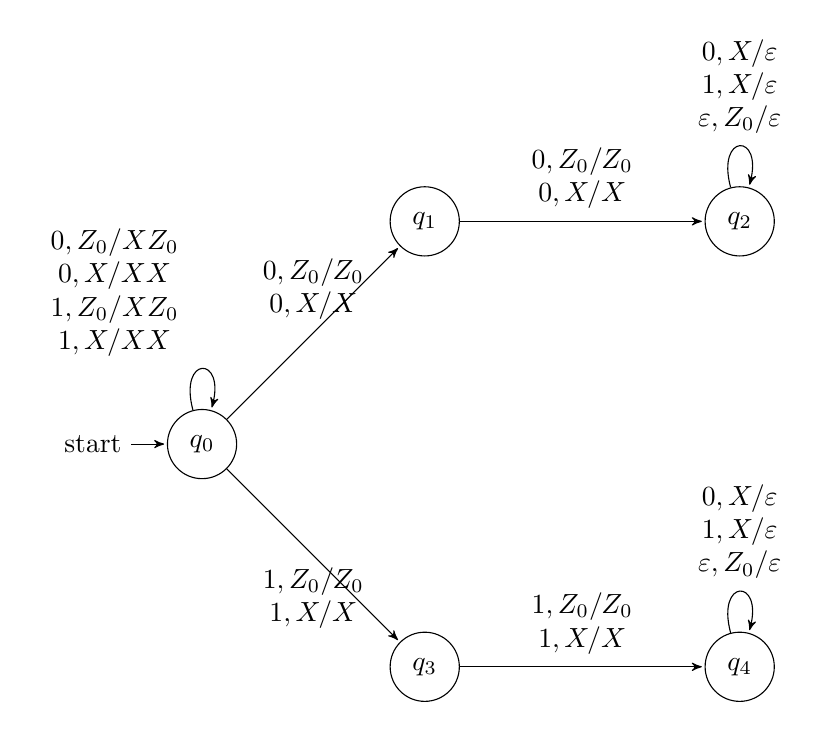
\begin{tikzpicture}[>=stealth',shorten >=1pt,auto,node distance=4cm]
 \node[initial,state] (q0) {$q_0$};
 \node[state,above right of=q0] (q1) {$q_1$};
 \node[state,right of=q1] (q2) {$q_2$};
 \node[state,below right of=q0] (q3) {$q_3$};
 \node[state,right of=q3] (q4) {$q_4$};

 \draw [->] (q0) edge [loop above] node [above left] {$
 \begin{array}{c}
 0, Z_0 / XZ_0 \\
 0, X / XX     \\
 1, Z_0 / XZ_0 \\
 1, X / XX
 \end{array}$} (q0)
 edge node [above] {$
 \begin{array}{c}
 0, Z_0 / Z_0 \\
 0, X / X
 \end{array}$} (q1)
 edge node [below] {$
 \begin{array}{c}
 1, Z_0 / Z_0 \\
 1, X / X
 \end{array}$} (q3)
 (q1) edge node {$
 \begin{array}{c}
 0, Z_0 / Z_0 \\
 0, X / X
 \end{array}$} (q2)
 (q2) edge [loop above] node {$
 \begin{array}{c}
 0, X / \varepsilon \\
 1, X / \varepsilon \\
 \varepsilon, Z_0 / \varepsilon
 \end{array}
 $} (q2)
 (q3) edge node {$
 \begin{array}{c}
 1, Z_0 / Z_0 \\
 1, X / X
 \end{array}$} (q4)
 (q4) edge [loop above] node {$
 \begin{array}{c}
 0, X / \varepsilon \\
 1, X / \varepsilon \\
 \varepsilon, Z_0 / \varepsilon
 \end{array}
 $} (q4);
 \end{tikzpicture}
 \caption{第二题}
 \end{figure}

 我们使用$X$字符来计数,
 而如果中间为$00$或$11$,
 那么就可以通过$q1, q2$或$q3, q4$来清空栈。
 当且仅当$00$或$11$为中心时,
 其两端的字符数才会相等,
 这样计数字符$X$才会清空。
\end{solution}

\section{第三题}
Convert the PDA $P = (\{p,q\},\{O,1\},\{X,Z_0\},δ,q,Z_0)$to a CFG,
if $\delta$  is given by:
\begin{enumerate}[fullwidth,itemindent=\parindent,label=(\arabic*)]
 \item $\delta(q,1,Z_0) = \{(q,XZ_0)\}$.
 \item $\delta(q,1,X) = \{(q,XX)\}$.
 \item $\delta(q,0,X) = \{(p,X)\}$.
 \item $\delta(q,ε, Z_0) = \{(q, \varepsilon)\}$.
 \item $\delta(p,1,X) = \{(p, \varepsilon)\}$.
 \item $\delta(p,0,Z_0) = \{(q, Z_0)\}$.
\end{enumerate}

\begin{solution}
 我们构造 CFG $G = (V, \{0, 1\}, P, S)$,
 其中$V = \{ [qXp] | q, p \in \{p, q\}, X \in \{0, 1\}\} \cup \{S\}$。
 而又有$\delta$函数,我们可以得出
 \begin{itemize}
 \item
 \begin{align*}
 S & \to [qZ_0q] | [qZ_0p]
 \end{align*}
 \item  $\delta(q,1,Z_0) = \{(q,XZ_0)\}$
 \begin{align*}
 [qZ_0q] & \to 1[qXq][qZ_0q] | 1[qXp][pZ_0q] \\
 [qZ_0p] & \to 1[qXq][qZ_0p] | 1[qXp][pZ_0p]
 \end{align*}
 \item $\delta(q,1,X) = \{(q,XX)\}$
 \begin{align*}
 [qZ_0q] & \to 1[qXq][qXq] | 1[qXp][pXq] \\
 [qZ_0p] & \to 1[qXq][qXp] | 1[qXp][qXp]
 \end{align*}
 \item $\delta(q,0,X) = \{(p,X)\}$
 \begin{align*}
 [qXq] & \to 0[pXq] \\
 [qXp] & \to 0[pXp]
 \end{align*}
 \item $\delta(q,ε, Z_0) = \{(q, \varepsilon)\}$
 \begin{align*}
 [qZq] & \to \varepsilon
 \end{align*}
 \item $\delta(p,1,X) = \{(p, \varepsilon)\}$
 \begin{align*}
 [pXp] & \to 1
 \end{align*}
 \item $\delta(p,1,X) = \{(p, \varepsilon)\}$
 \begin{align*}
 [pXp] & \to 1
 \end{align*}
 \item $\delta(p,0,Z_0) = \{(q, Z_0)\}$
 \begin{align*}
 [pZ_0q] & \to 0[qZ_0q]
 \end{align*}
 \end{itemize}

 化简后有
 \begin{align*}
 S       & \to [qZ_0q]                     \\
 [qZ_0q] & \to 1[qXp][pZ_0q] | \varepsilon \\
 [qXp]   & \to 1[qXp][pXp] | 0[pXp]        \\
 [pZ_0q] & \to 0[pZ_0q]                    \\
 [pXp]   & \to 1
 \end{align*}
\end{solution}

\end{document}
